\documentclass[a4paper,11pt]{scrartcl}
\usepackage[utf8x]{inputenc}
\usepackage{lmodern,textcomp}
\usepackage{amsmath,amsfonts}

\usepackage{authblk}
\usepackage{graphicx}
\usepackage{enumitem}
\setdescription{style=nextline}

\newcommand{\usd}{\text{\textdollar}}
\newcommand{\ee}{\text{\texteuro}}
\newcommand{\amo}{$\mathbb{A}$\ }
\newcommand{\amom}{\mathbb{A}}

% title
\title{Economy Simulation for PoS- or DPoS-based Blockchains}
\date{November 22, 2019}
\author{Yeon-Hyeong Yang}
\affil{AMO Labs}

\begin{document}

\maketitle

\begin{abstract}
	Summary of what we did.

	This paper describes a series of simulation results of blockchain economy.
	The simulation model is defined using classic economy theories modified and
	adapted to blockchain-specific environments.
\end{abstract}

\section{Introduction}
What will be discussed. Why it is important. What approach we use.

\section{Terms and Definitions}
In this section, we explain terms and definition we need in the blockchain
economy simulation. Some of the terms are defined in the AMO blockchain
protocol, but we also need to borrow terms from classic economics textbooks.

\subsection{Blockchain}
In order for a blockchain to operate as \emph{blockchain} we need the following
concepts.

\subsubsection{Transaction}
A transaction is an atomic unit of state change. In canonical terms, a
transaction is realization of a user's intention. In out simulation users tend
to generate transactions based on the output level of the AMO economy. For one
unit of good to be traded, we need 3 transactions to complete the cycle of one
trade: seller registers a good, buyer request a good with pledged payment,
seller grant the request collecting the payment. In this simulation, we set one
unit of good to be a good with the value of one dollar. So, if the total output
$Y$ of the economy is worth 1,000 dollars, then the number of newly generated
transactions, $T_N$, would be 3,000. 

Another factor that affects the transaction generation is the transaction fee
level. If the transaction fee is too high, some of the users would give up the
transaction considering that the cost is higher than the benefit of the trade.
This effect summarizes to the following relation:
\begin{equation}
	T_N' = T_N \times \frac{F_C}{F + F_C},
\end{equation}
where $F_C$ is called a \emph{fee cap} and given as one of the domain
parameters.

\subsubsection{Block}
A grouped collection of transactions.
block size: Maximum number of transactions in a block

\begin{description}
	\item[user account]
		An entity who generates transactions. sometimes simpley denoted as an
		\emph{account}
	\item[validator]
		An entity who collects transactions and form a block
	\item[(AMO) coin]
		Modern blockchain protocols run with native coin system
	\item[stake]
		Locked as a stake
	\item[transaction fee]
		Given to a validator
	\item[transaction reward]
		Newly minted and given to a validator
\end{description}

\subsubsection{Taxonomy of coins}
\begin{description}
	\item[active coins]
		Reside in a user account and ready to be transferred or used.
	\item[dormant coins]
		Reside in a validator's account and ready to be transferred or used,
		but the validator wants pile up these coins rather than use it.
	\item[lost coins]
		Reside in a user account, but the user lost his/her key.
\end{description}

\subsection{Blockchain Economy}
Terms borrowed from classic economics theory.

\subsubsection{Money Supply}
Money supply is sum of all monetary assets that can be spent freely, and have
high liquidity. We set money supply in AMO economy as simply the sum of all
active coins. \emph{Money} in AMO economy consists of active coins, dormant
coins, lost coins and stakes. By definition, dormant coins are viable to be
spent on demand but the owners are not willing to spend in near future. Lost
coins are not viable to be spent permanently due to the user key loss. Stakes,
or staked coins cannot be transferred to other account, so they cannot function
as cash. Therefore, only active coins are considered as \emph{cash} in our
economy simulation. Since we are not considering any sophisticated financial
authorities, money supply in AMO economy equals to the sum of all active coins.

\subsubsection{money demand}
Demand

\subsubsection{Interest Rate}
Interest rate is a rate of return from invested money to non-cash asset.
According to [1] monetary assets such as cash does not provide interest. It is
true for the AMO economy. If someone store their AMO coins in their accout,
they just sit there. Without any other effect, user account balance will not
change. The only possible asset which provide an interest in AMO blockchain is
a stake. Validators and delegators get reward via staking or delegation. Given
the fixed reward rate, the total reward amount is calculated from number of
transactions processed. So the interest rate of stake or delegated stake can be
directly calculated from the sum of all stakes and delegated stakes and the
number of transactions processed.

\subsubsection{exchanse rate}
Price of one currency quoted as another currency
\subsubsection{exchange rate expectation}
Future expectation of the exchange rate
\subsubsection{production output}
Total value of goods ready to be traded
\subsubsection{price level}
Average price of one unit of goods
\subsubsection{money velocity}
Velocity at which one unit of money being circulated

\section{Simulation Model}
We will use the symbol ``\amo'' for AMO in mathematical expressions, although
the actual currency denominator adapted in various cryptocurrency market is
just ``AMO''.

\subsection{Simulation Steps}
State, history of state, state transition, unit of time

\subsection{Domain Parameters}
\begin{description}
	\item[$T_B$] Maximum number of transactions in a block
	\item[$R_\$$] Interest rate of the outer world, i.e. dollar-based economy
	\item[$P_\$$] Price level of the outer world, i.e. dollar-based economy
	\item[$Y_{GDP}$] GDP function for AMO economy
	\item[$V$] Velocity of AMO coin
	\item[$r$] Reward given to a validator for processing one transaction
\end{description}

\subsection{State Variables}
The internal state of simulation model is a collection of state variables. The
simulation state includes the following variables:
\begin{description}
	\item[$T_P$] Number of pending transactions at the end of the current
		simulation step
	\item[$F$] Average transaction fee (\emph{measured in AMO})
	\item[$M$] Sum of all coins (\emph{measured in AMO}) \\
		$= M^A + M^D + M^L + S$
	\item[$M^A$] Sum of all active coins (\emph{measured in AMO})
	\item[$M^D$] Sum of all dormant coins (\emph{measured in AMO})
	\item[$M^L$] Sum of all lost coins (\emph{measured in AMO})
	\item[$S$] Sum of all staked coins (stakes for validators and
		delegated stakes for delegators) (\emph{measured in AMO})
	\item[$R_\amom$] Interest rate of the AMO economy
	\item[$P_\amom$] Price level of the AMO economy
	\item[$Y$] Production yield of the AMO economy during the current
		simulation step (\emph{measured in dollar})
	\item[$E_{\usd/\amom}$] Exchange rate quoted as dollar per one AMO
		(\emph{dollar price of one AMO})
\end{description}

\subsection{Intermediate Variables}
These variables are not part of state variables. They are calculated from state
variables from previous step and used in calculating state variables for the
next step.

\begin{description}
	\item[$T_N$] Number of newly generated transactions during the current
		simulation step
	\item[$T$] Number of processed transactions during the current simulation
		step
	%\item[$M^s$] Aggregate money supply of the AMO economy
	\item[$M^d$] Aggregate money demand of the AMO economy
	\item[$E^e_{\$/\amom}$] Exchange rate expected after one year from
		current simulation step quoted as dollar per one AMO
		(\emph{dollar price of one AMO})
\end{description}

\section{Economic Assumptions}
In this section, we describe the market dynamics when observed in a few
economical viewpoints. Most of the rudimentary theoretical backgrounds were
borrowed from classic economics textbooks. Major contribution of this section
is to adapt those theories to the specific environment of AMO blockchain
economy (or any Pos- or DPoS-based blockchain economy).

\subsection{Local Money Market}
Recall symbols:
\begin{description}
	\item[$M^d$] Money demand
	\item[$M^s$] Mopey supply
	\item[$P_\amom$] Price level of the AMO economy
\end{description}

\subsubsection{Money and Price Level}
Relation between money demand and supply in the local money market:
\begin{eqnarray}
	M^d = P_\amom \times L(R_\amom,Y) \label{localdemand} \\
	M^s = M^A \\
	\text{equilibrium at\ } M^s = M^d \\
	\implies M^A = P_\amom \times L(R_\amom,Y) \label{eq1}
\end{eqnarray}

\textbf{TODO: implications of the above equation.}

The production output $Y$ is given by the GDP function $Y_{GDP}$. $R_\amom$ is
calculated from $S$, $T$ and fixed $r$. Since the reward in AMO blockchain is
for transactions, not blocks, $T$ is in turn depends on $Y$. So, it is natural
to think that $L(R_\amom,Y)$ is a function $L'$ of $S$ and $Y$, i.e. $L'(S,Y)$.
Therefore,
\begin{equation}
	M^A = P_\amom \times L'(S,Y) \label{eq2}
\end{equation}
Note that $M^A$ also depends on $S$. So \eqref{eq2} is an equilibrium
condition for $P_\amom$ and $S$. From this argument, we can use the above
condition \eqref{eq2} in two ways:
\begin{enumerate}
	\item calculate long-run change of $P_\amom$ based on the current value of
		$S$ and $Y$
	\item calculate short-run change of $S$ based on the current value of
		$P_\amom$ and $Y$
\end{enumerate}

In order to do that, we need to decide the function $L$ or $L'$ (called
liquidity preference function). Among the various number of theories, we took 2
models out of them from the next section.

\subsubsection{Liquidity Function} \label{liquidity}
%%%%%%%%%%%%%%%%%% Fisher's Exchange Equation
Fisher's exchange equation[3] is
\begin{equation}
	M \times V = P \times Y, \label{eq:fisher}
\end{equation}
where $V$ is a money velocity. When we combine \eqref{eq1} with
\eqref{eq:fisher}, we get
\begin{equation}
	L(R, Y) = Y / V. \label{eq3}
\end{equation}
This is simple and neat, but does not depend on interest rate $R_\amom$.

%%%%%%%%%%%%%%%%%% Baumon-Tobin Model
Baumon-Tobin model[4] is
\begin{equation}
	L(R, Y) = \sqrt{\frac{cY}{2R}}, \label{eq4}
\end{equation}
where $c$ is the cost of converting between assets, such as money(AMO coin) and
interest-bearing assets(stakes).
When we grab the ideas from \eqref{eq3} and \eqref{eq4}, we can say that
\begin{eqnarray}
	V \times L(R, Y) = \sqrt{\frac{cY}{2R}} \\
	\text{Thus,\ } L(R, Y) = \frac{1}{V} \times \sqrt{\frac{cY}{2R}} \label{eq5}
\end{eqnarray}
By combining \eqref{localdemand} and \eqref{eq5} we get the following.
\begin{eqnarray}
	M^d = P_\amom \times \frac{\sqrt{\frac{cY}{2R_\amom}}}{V}
\end{eqnarray}
We can calculate excess money supply from $M^A - M^d$, or money supply in short
from $M^d - M^A$. The excess money supply tends to be converted into
interest-bearing assets such as stakes, while the money supply in short tends
to be compensated from stakes.

Local money market moves towards the equilibrium point described by
\eqref{eq1}. From this, we can calculate long-run change of price level of AMO
economy. By combining \eqref{eq1} and \eqref{eq5}, we get equilibrium point of
long-run price level.
\begin{equation}
	P'_\amom = M^A \times \frac{V}{\sqrt{\frac{cY}{2R_\amom}}}
\end{equation}

\subsection{Currency Exchange Market}

\subsubsection{Purchasing Power Parity(PPP) Condition}
Law of One Price

The \textbf{purchasing power parity(PPP)} condition[2].
\begin{eqnarray}
	\text{equilibrium at\ } E_{\usd/\amom} = P_\usd / P_\amom \label{eq:3}
\end{eqnarray}

\textbf{TODO: implications of the above equation. with the law of one price.
with free trade condition.}

Given $P_\usd$, we can use the above condition \eqref{eq:3} to calculate
expected future exchange rate in the long run ($E^e_{\usd/\amom}$).

\subsubsection{Interest Parity Condition}
The \textbf{interest parity} condition[1] states a condition when the currency
exchange market is in equilibrium. We have two economy systems: dollar system
and AMO system. Each of the systems has its own domestic currency, dollar(\usd)
for dollar system, and AMO coins for AMO system. We can think of a currency
exchange market where dollar and AMO coins are bought and sold. When we denote
$E_{\usd/\amom}$ as a dollar price of one AMO coin, the currency exchange market
is in equilibrium when the following condition holds.
\begin{eqnarray}
	\text{dollar return rate} = R_\usd \\
	\text{AMO return rate} = R_\amom + \frac{(E^e_{\usd/\amom} - E_{\usd/\amom})}
	{E_{\usd/\amom}} \\
	\text{equilibrium at\ } \text{dollar return rate} = \text{AMO return rate} \\
	\implies R_\usd = R_\amom + \frac{(E^e_{\usd/\amom} - E_{\usd/\amom})}
	{E_{\usd/\amom}} \label{eq:2}
\end{eqnarray}
$R_\usd$ is the interest rate of the dollar system(we can say just
\emph{outer world}), $R_\amom$ is of the AMO system, $E_{\usd/\amom}$ is the
dollar price of one AMO, and $E^e_{\usd/\amom}$ is the expected dollar price of
one AMO after one year from now.

\textbf{TODO: implications of the above equation.}

We use the above condition \eqref{eq:2} to calculate short-run exchange rate
change. Note that $R_\usd$ is given as a domain parameter, $R_\amom$ is
calculcated from $S$, $T$ and $r$.
\begin{equation}
	E'_{\usd/\amom} = \frac{E^e_{\usd/\amom}}{R_\usd - R_\amom + 1}
\end{equation}

\section{Other Assumptions}

\subsection{Transactions}

\subsubsection{Generation}
\subsubsection{Fee}
In AMO blockchain protocol, a transaction fee is up to the sender of the
transaction. It may be zero, or non-negative but there is no obligation to pay
a fee to the validator who processes the transactions. When there is enough
room in blocks for newly generated transactions, user may set the fee to be
zero, and even in that case validators would willing to process them to get tx
reward from them.

However, when the number of transactions awaiting to be included in a block is
relatively high (higher than the block size limit), some users want to non-zero
fee to get express service for their transactions. Once again, a transaction
fee is up to the sender fo the transaction, and there is no exact formula to
calculate a fee. Generally, it is decided in the market, but the decision is
collective and there is no clear supply-demand properties here. So, to simulate
the market, we assume the following relation.
\begin{eqnarray}
	t_\text{waiting} = T_P / T_B \\
	F = c P_\amom \times t_\text{waiting}
\end{eqnarray}
Recall that $T_P$ is the number of pending transactions, and $T_B$ is the
maximum number of transactions in a block. So, $T_P / T_B$ is the number of
blocks required before the last transaction in the pending queue to be included
in a block. $c$ is an arbitrary constant. Actual desired fee is acquired by
multiplying this with the price level of AMO economy $P_\amom$.

\subsubsection{Suppressing Transactions}

\subsubsection{Processing}
Due to the limit of the block size and other environmental factors, it may not
be possible to process all the newly generated transactions right away.
Transactions spread out from the user's client program, but it takes time for
the transactions to reach the validator node which would include them in a
block. Some quick, some slow. We mark the portion of the transactions in the
network to be \emph{lazy}. Lazy transactions will not be processed in the
current simulation step, and carried on to the next step via $T_P$. In addition
to this, it is possible for a transaction to lose the chance to be included in
a block due to the block size limit. These transactions will be carried on to
the next step via $T_P$ also.

\subsection{Natural Depeletion}
Since there is no perfect system, there may be mishaps and inefficiency and
unexpected crash of a certain blockchain node. To simulate this factor, we
introduced a depletion logic. The logic is simple. It is applied at the end of
every simulation step.
\begin{enumerate}
	\item{cast out small portion of pending transactions($T_P$)}
	\item{convert small portion of dormant coins($M^D$) to lost coins($M^L$)}
\end{enumerate}
First one is to simulate the accidental events in the blockchain node's
mempool(pool of transactions awaiting to be processed), and the second one is
to simulate the accidental asset loss due to the user key loss. Note that the
dormant coins are the most inactive assets in this simulation. So, the
possibility of \emph{accident} is also relatively high.

\section{State Transition}
Since the simulation model is a kind of a state machine, a state in a
particular step is a result of a state stransition function upon a state of the
previous step. General principle for calculating the next state is to predict
an equilibrium point based on previous state and then apply slow or fast
approach functions accordingly.

\subsection{Approach Functions}
There are some state variables calculated directly from the previous state. But
some of the state variables represents activies from various market actors.
Some of them changes fast but with slight damping effect, and some of them
changes slow even if the movement pressure is high. We use the two types of
approach functions to simulate these types of changes. The fast approach
function represents short-run changes such as exchange rate change, and the
slow approach function represents long-run chagnes such as price level change.
The approach functions take two input parameters, the current and the target,
and output one result value. These functions also utilizes the simulation step
size from the domain parameter.

\subsubsection{Approach Unit Function}
An approach function $f_\tau(\text{current}, \text{target}, \text{time})$ has
the following characterstics:
\begin{itemize}
	\item{$f_\tau(a, a_\tau, 0) = a$}
	\item{$f_\tau(a, a_\tau, \tau) \approx a_\tau$}
	\item{When we define $\delta_t = f_\tau(a, a_\tau, t + \Delta) - f_\tau(a,
			a_\tau, t)$, then $|\delta_t| > |\delta_{t+c}|$}
	\item{$f_\tau(a, a_\tau, t+\Delta) = f_{\tau-\Delta}(a_\Delta, a_\tau,
		t)$}, where $a_\Delta = f_\tau(a, a_\tau, \Delta)$.
\end{itemize}

One of the method to construct such an approach function is as follows:
\begin{enumerate}
	\item{find an appropriate unit approach function $\delta_1(t)$ such that}
		\begin{itemize}
			\item{$\delta_1(0) = 1$}
			\item{$\delta_1(1) \approx 0$}
			\item{the derivative $\delta_1'(t)$ is negative and monotonic
				increasing}
			\item{$\delta_1(\Delta) / \delta_1(0) = 
				\delta_1(2\Delta) / \delta_1(\Delta)$}
		\end{itemize}
	\item{define an approach function
		$f_\tau(a, a_\tau, t) = a_\tau - (a_\tau - a) \times \delta_1(t/\tau)$}
\end{enumerate}
The remaining work is to find an appropriate unit approach function. One of the
candidates is an exponentially decreasing function $c^{-t}$ for some constant
$c$. For the constraint $\delta_1(1) \approx 0$, $c^{-1}$ should be very close
to the value 0. If we say 0.01 is sufficiently close to 0 (when compared to the
starting value of 1), then $c$ should be greater than or equal to 100. Thus,
we set our approach function $f_\tau(a, a_\tau, t)$ to be $a_\tau - (a_\tau -
a) \times 100^{-t/\tau}$.

\subsubsection{Short-Run Changes}
State variables with short-run change move to their destination(usually the
equilibrium point) rather quickly. All else equal, these variables reach their
destination in a few siumulation days. Affected variables are $S$, $F$ and
$E_{\usd/\amom}$. For this purpose, we set $\tau$ to be 3 days. Of course, the
input parameter $t$ must be adjusted to be in scale of days.

\subsubsection{Long-Run Changes}
State variables with long-run chagne move to their destination rather slowly.
All else equal, these variables reach their destination in a year roughly.
Affected variables are $P_\amom$. For this purpose, we set $\tau$ to be 1 year.
Of course, the input parameter $t$ must be adjusted to be in scale of years.

\subsubsection{Inertia and Momentum}

\subsection{Economy Output}
The GDP function gives $Y$ value at each simulation step according to the
progression of the simulation, i.e. the number of simulation steps elapsed. It
is a scheduled function and given as part of domain parameters, so it has no
dependency to the state variables. This function is used to write simulation
scenarios depicting various market trends and business environment changes.

\subsection{Stake}
Calculate money demand for AMO coin by the method described in
\ref{liquidity}. Calculate excess money supply by $M^A - M^d$. Apply the
short-run change function with the current value as $S$, the target value as
$S + M^A - M^d$. Let the output from the change function to be $\Delta$.

Set $S_i = S_{i-1} + \Delta$ and $M^A_i = M^A_{i-1} - \Delta$.

\section{Simulation Results}

\subsection{Scenarios}
We prepared 3 scenarios for the AMO economy simulation regarding the market
trends:
\begin{enumerate}
	\item{Constant weak output} (section \ref{sc1})
	\item{Constant weak output with additional positive expectation} (section \ref{sc1.1})
	\item{Constant high output} (section \ref{sc2})
	\item{Constant high output with additional positive expectation} (section \ref{sc2.1})
	\item{Start weak and grows} (section \ref{sc3})
	\item{Start weak and grows with additional positive expectation} (section \ref{sc3.1})
\end{enumerate}
All the scenarios have identical initial state except market trend. The initial
state is as the following:
\begin{itemize}
	\item{total coins($M$) = 20,000,000,000 AMO}
	\item{active coins($M^A$) = 19,000,000,000 AMO}
	\item{dormant coins($M^D$) = 0 AMO}
	\item{lost coins($M^L$) = 0 AMO}
	\item{stakes($S$) = 100,000,000 AMO}
	\item{interest rate of AMO($R_\amom$) = 0.1}
	\item{interest rate of USD($R_\usd$) = 0.02 (stays constant)}
	\item{price level of AMO world($P_\amom$) = 1}
	\item{price level of USD world($P_\usd$) = 1 (stays constant)}
	\item{exchange rate as dollar per AMO($E_{\usd/\amom}$) = 0.0005}
\end{itemize}

\textbf{TODO: Additional positive expectation.}

\subsection{Scenario 1: Constant Weak Output}
\label{sc1}

\begin{figure}[hbt!]
	\centering
	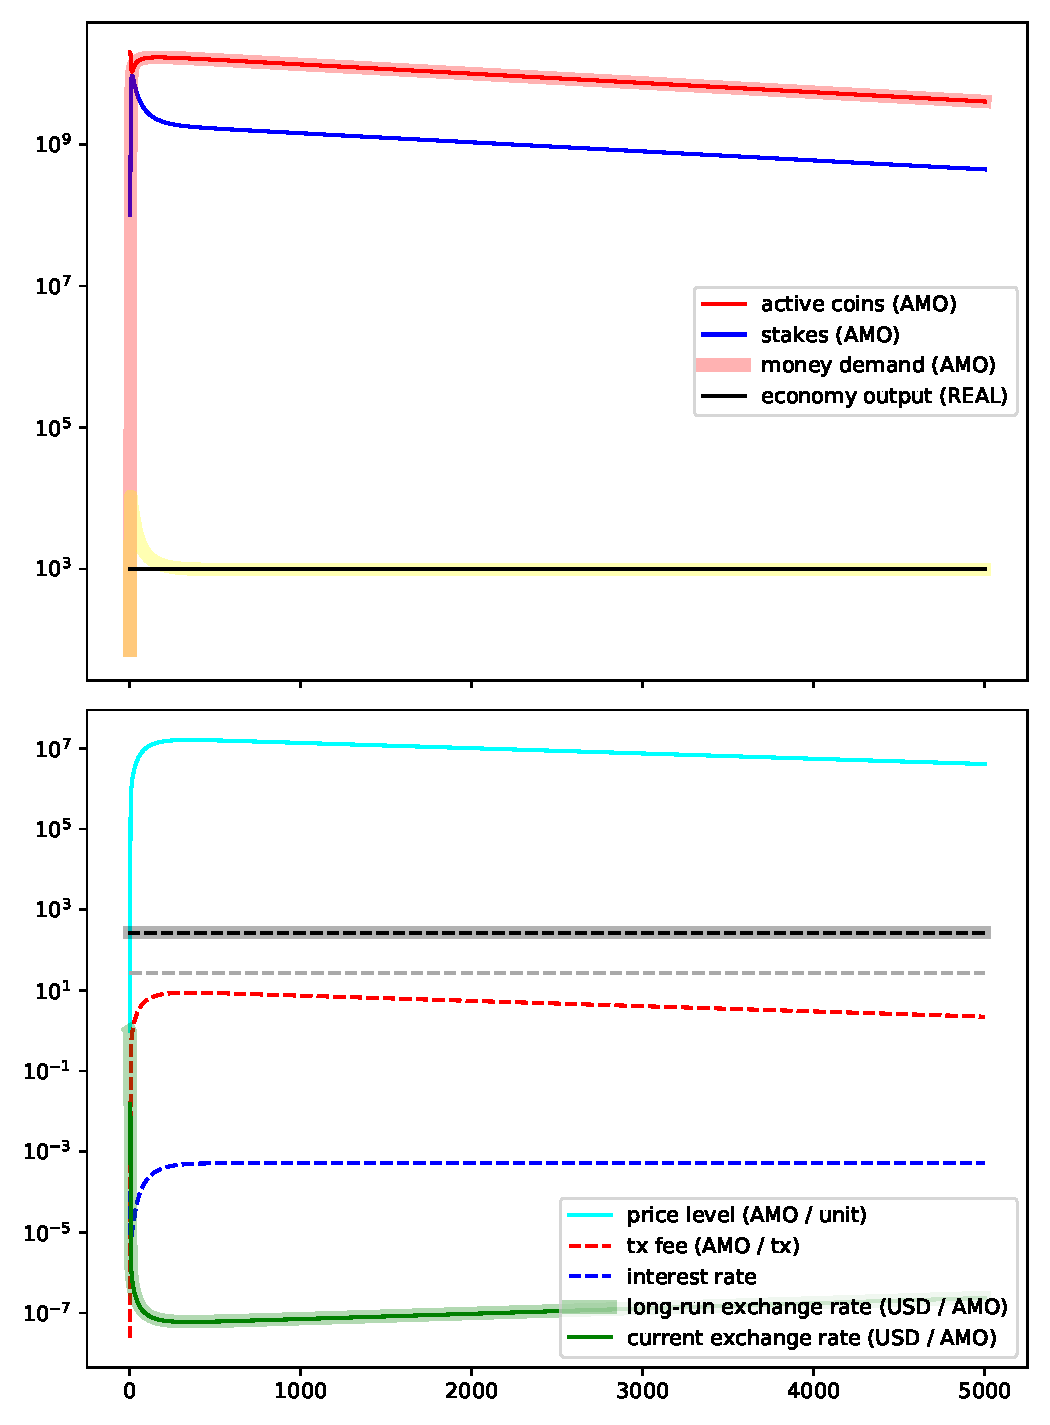
\includegraphics[width=0.8\textwidth]{fig/fig1.pdf}
	\caption{(scenario 1) constant weak output}
	\label{fig:sc1}
\end{figure}

Figure \ref{fig:sc1} shows the simulation result of scenario 1 over the time
span of 5,000 days. The upper part of the figure shows the trend of assets in
AMO blockchain economy, while the lower part shows the various metrics
calculated from the blockchain state. The most important line here is the
output trend. We set the output to be constant value 1,000, meaning 1,000\$
worth of trade during 1 year. The output, together with price level, decides
the settling points for various assets. In a short run, the price level is
considered fixed, and it decides the money demand along with the interest rate.
Money demand controls the amount of stakes and active coins. Stakes are
changing as a medium-run variable(slower than short-run variables, but faster
than long-run variables) according to the money demand. With stakes changing in
medium-run pace, the price level is adjusted in a long-run pace. Once the
stakes and active coins settle down first, the price level is adjusted
gradually. Since short-run and medium-run variables settle down according to
the long-run variable(price level), all the other metrics now follows the
gradual change of the price level.

One thing to note is that the price level is high since the output is low. This long-run price level is driving overall pace of all the other variables.

The exchange rate is a short-run variable, but there is also an expected
exchange rate in the long-run. After the short-run exchange rate settles down
to some point quickly, it follows the long-run change expected exchange rate,
which is determined by the price level. You can see the broad green
line(expected exchange rate) is the upside down image of the cyan line(price
level).

In this scenario, everything looks rather gloomy: too much active coins, low
exchange rate(bad for coin holders regarding coin value), and high price
level(bad for real customers).

\subsection{Scenario 1 with Additional Positive Expectation}
\label{sc1.1}

\subsection{Scenario 2: Constant High Output}
\label{sc2}

\begin{figure}[hbt!]
	\centering
	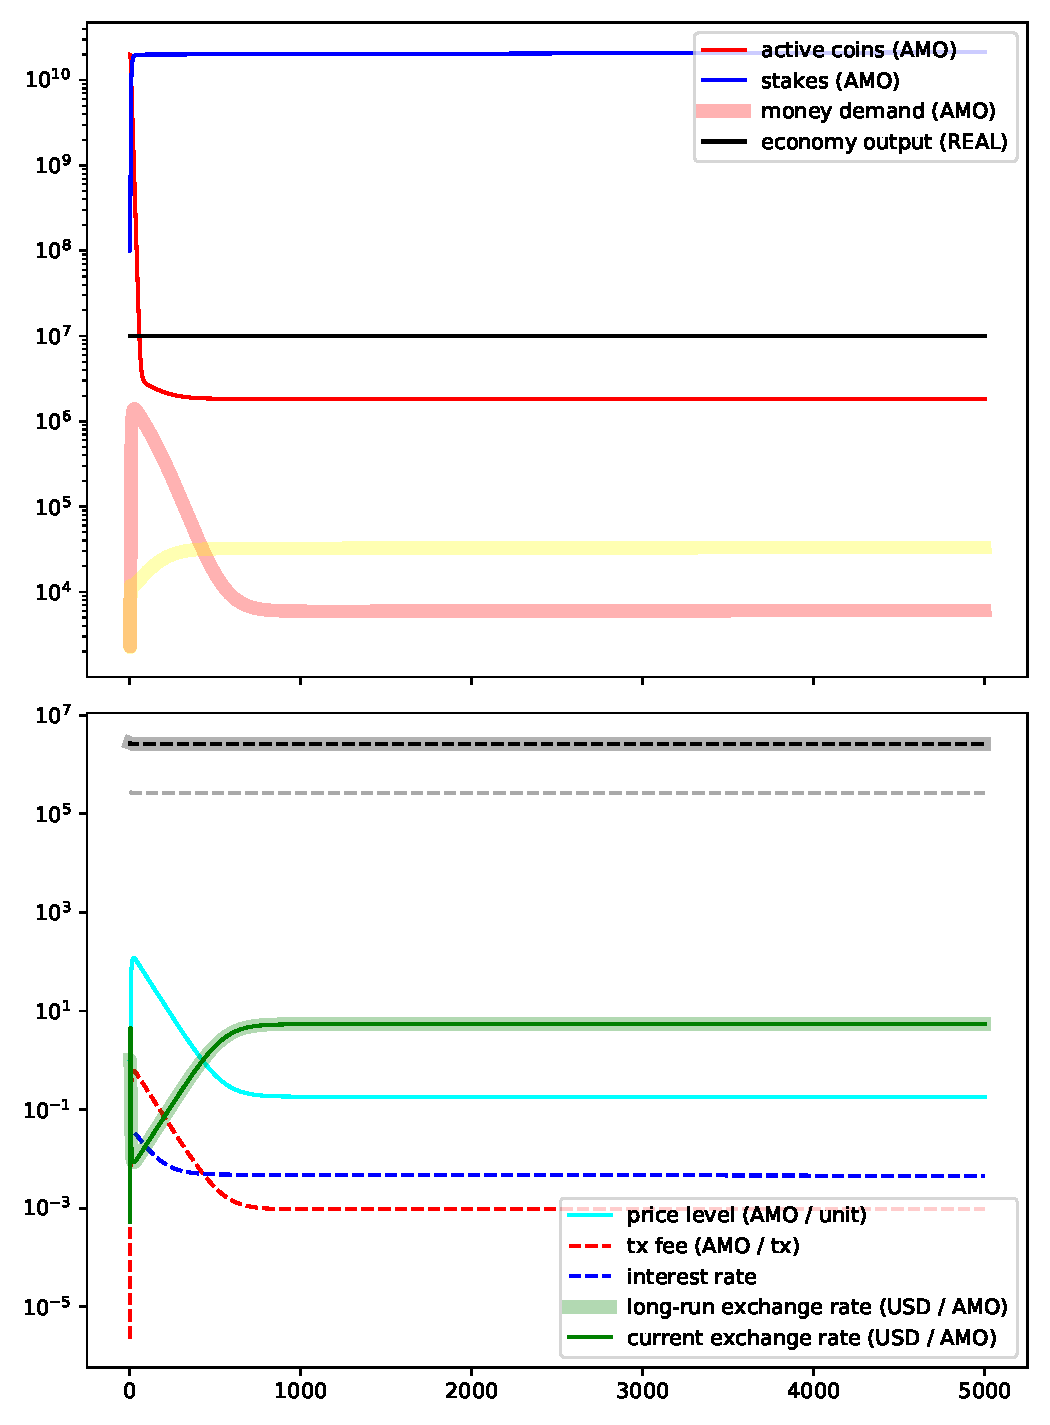
\includegraphics[width=0.8\textwidth]{fig/fig2.pdf}
	\caption{(Scenario 2) Constant high output}
	\label{fig:sc2}
\end{figure}

Figure \ref{fig:sc2} shows the simulation result of scenario 2 over the time
span of 5,000 days. We set the output to be constant value 10,000,000, meaning
10,000,000\$ worth of trade during 1 year, which is 10,000 times higher than
the scenario 1. The dynamics of the economy is prettey much the same as the
scenario 1, but with high output, the price level is lower than the scenario 1
by a factor of 8.

\subsection{Scenario 2 with Additional Positive Expectation}
\label{sc2.1}

\subsection{Scenario 3: Start Weak and Grows}
\label{sc3}

\begin{figure}[hbt!]
	\centering
	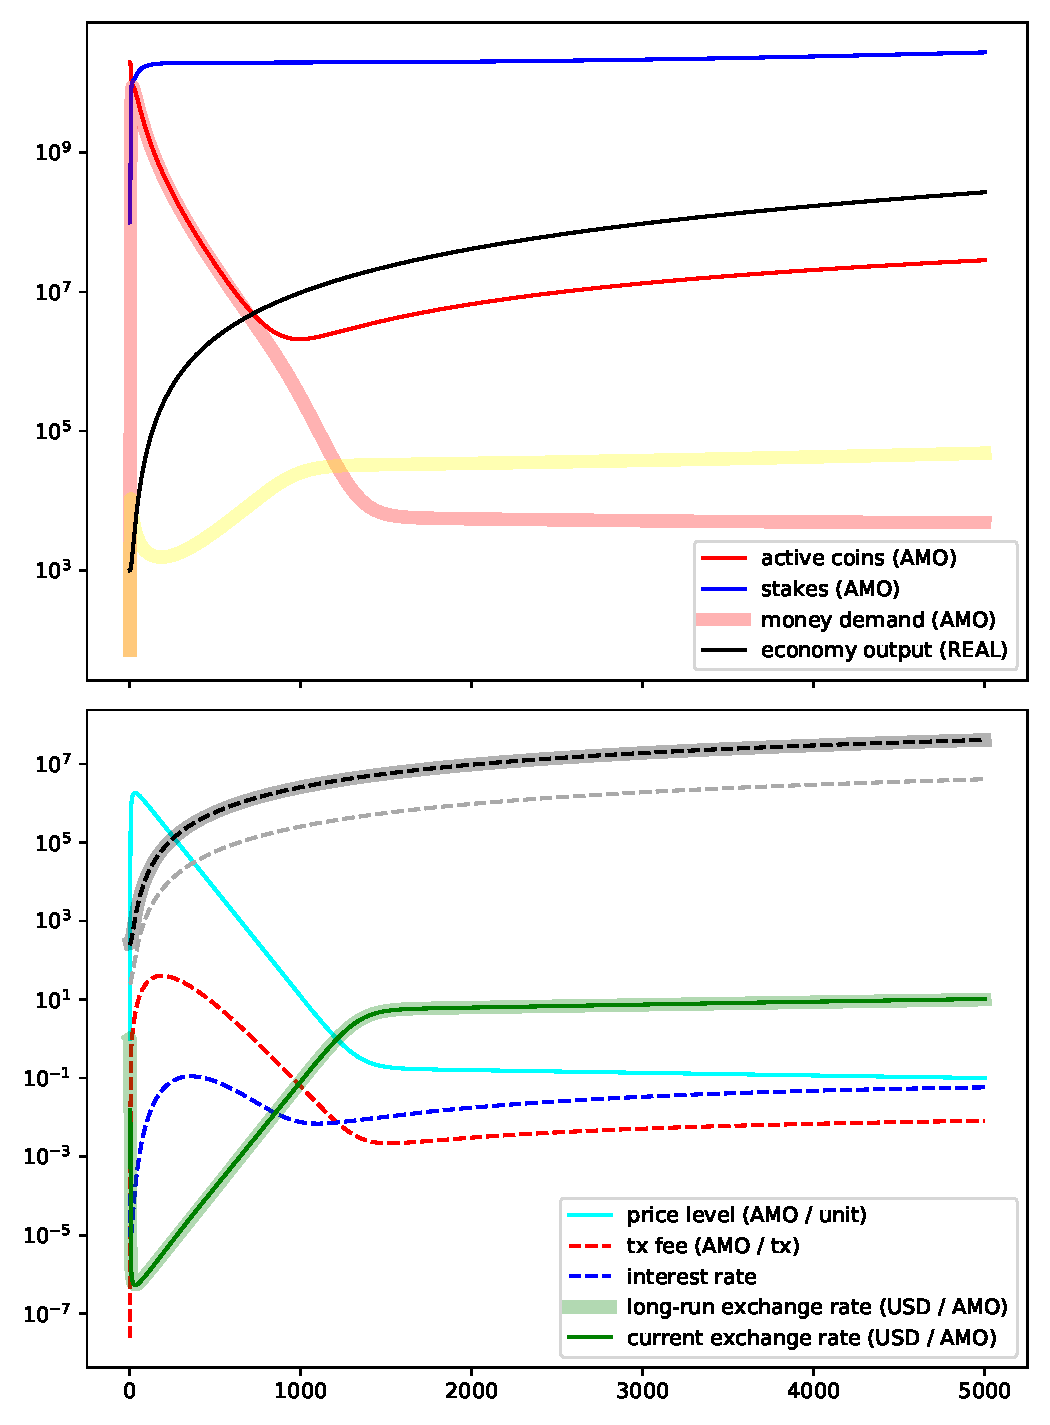
\includegraphics[width=0.8\textwidth]{fig/fig3.pdf}
	\caption{(Scenario 3) Start weak and grows}
	\label{fig:sc3}
\end{figure}
We use the following output function:
\begin{equation}
	c_2x^2 + c_1x + c_0,
\end{equation}
where $c_2$, $c_1$ and $c_0$ are chosen to be 10,000, 10,000 and 1,000,
respectively. The output of the function is translated as dollar amount of
trades during one year.

Figure \ref{fig:sc3} shows the simulation result of scenario 3 over the time
span of 5,000 days.

\subsection{Scenario 3 with Additional Positive Expectation}
\label{sc3.1}

\end{document}
